\scanpage{26}

Ce théorème ramène essentiellement l'étude de $\mathrm{Pl}_{\mathrm{isot}}^\alpha$ à celle de $\mathrm{Pl}_{\mathrm{isot}}(U_\alpha,S)$. Pour faire cette étude, on doit pouvoir donner un procédé pour décrire combinatoirement $U_\alpha$ en termes de $\alpha$. Notons

\uline{Prop} $U_\alpha-X=\unsure{V|W|\mathcal V}_\alpha$ a des composantes connexes \inserted{$V_\alpha^i$} qui sont des produits $\underset{\text{cercle}}{S^1}\times\deleted{\unsure{]0,1[}}[1,2[$ \deleted{et \unsure{$V_\alpha$} \illegible{1} le bord de $U_\alpha$ est le filtre des} \inserted{avec $\mathrm{bord}(U_\alpha)\cap V_\alpha^i\simeq S^1\times\{1\}$}, les voisinages de $X$ dans $U_\alpha$ induisant sur $V_\alpha^i$ le filtre des voisinages de $S^1\times\{1\}$ dans $S^1\times]0,2[$.

% slanted
\margin{le nb des $V_\alpha^i$ est $b_1(X)+1$ si $X$ connexe non vide ? Cela donnerait $b_1(X)+b_0(\unsure{x|X})$ dans le cas général ?}
\figure{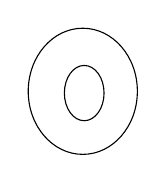
\begin{tikzpicture}[scale=.45]
\draw (0,0) ellipse (1.54 and 1.78); \draw (.04,-.05) ellipse (.56 and .78);
\end{tikzpicture}}
\deleted{Donc}\quad\deleted{\unsure{Déf}}

Donc la surface $S$, pour un plongement donné de $U_\alpha$, peut se décrire comme \deleted{\unsure{$U_\alpha$|$\mathcal U_\alpha$}} déduite de $U_\alpha$ en lui collant une variété \inserted{orientée} à bord $U'$ [compacte \unsure{sss|ssi} $S$ est compacte] \deleted{\unsure{à|---}} savoir $\overline{S-\varphi(U_\alpha)}$ --- à $U_\alpha$, par un isom \deleted{\unsure{de}} $bU'_{\unsure{\alpha}}$ avec $-bU_\alpha\simeq$

\figure{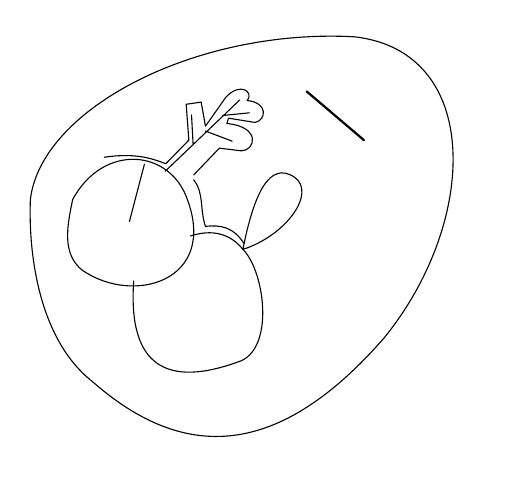
\begin{tikzpicture}[scale=.68,line cap=round,line join=round]
\draw (-3.4,.70) .. controls (-3.2,2.4) and (-.3,3.9) .. (2.65,3.74) .. controls (5.05,3.47) and (4.97,.29) .. (3.21,-1.88) .. controls (1.25,-4.13) and (-.51,-4.22) .. (-2.24,-2.70) .. controls (-3.21,-1.94) and (-3.44,-.40) .. (-3.4,.70);
\draw (-2.61,.70) .. controls (-2.04,1.76) and (-.78,1.65) .. (-.46,.68) .. controls (.08,-.82) and (-1.47,-1.28) .. (-2.43,-.62) .. controls (-2.82,-.31) and (-2.71,.22) .. (-2.61,.70);
\draw (-1.47,-.82) .. controls (-1.58,-2.4) and (-.87,-2.84) .. (.54,-2.31) .. controls (1.16,-2.03) and (.97,-.63) .. (.57,-.23) .. controls (.28,.13) and (-.10,.12) .. (-.41,.02);
\draw (.57,-.23) .. controls (1.38,.03) and (1.95,.83) .. (1.53,1.12) .. controls (1.06,1.43) and (.77,.79) .. (.57,-.23);
\draw (-1.27,1.36)--(-1.55,.29);
\draw (-2.02,1.49) .. controls (-1.37,1.59) and (-1.05,1.43) .. (-.87,1.37) --(-.44,1.81)--(-.49,2.48)--(-.21,2.52)--(-.13,2.07)--(.25,2.61) .. controls (.53,2.91) and (.78,2.70) .. (.65,2.55) .. controls (1.04,2.51) and (1.01,2.19) .. (.80,2.14)--(.30,2.22)--(.27,2.12) .. controls (.92,2.06) and (.80,1.61) .. (.54,1.61)--(.13,1.66)--(-.35,1.16);
\draw (-.88,1.23)--(.51,2.56) (-.36,1.72)--(-.39,2.28) (-.13,1.98)--(.37,1.79) (.19,2.27)--(.69,2.32);
\draw (-.35,1.07) .. controls (-.15,.81) and (-.24,.52) .. (-.13,.20) .. controls (.15,.23) and (.39,.19) .. (.59,-.12);
\draw[thick] (1.76,2.72)--(2.83,1.81);
\end{tikzpicture}}
\figure{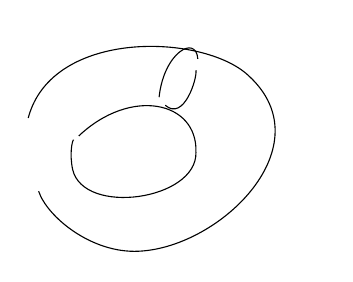
\begin{tikzpicture}[scale=.60]
\draw (-2.45,.63) .. controls (-1.95,2.53) and (1.28,2.42) .. (2.22,1.52) .. controls (3.82,.05) and (1.63,-2.11) .. (-.11,-2.19) .. controls (-1.11,-2.24) and (-2.05,-1.46) .. (-2.23,-.92);
\draw (-1.38,.25) .. controls (-.28,1.29) and (1.14,.99) .. (1.10,-.10) .. controls (1.12,-1.11) and (-1.28,-1.45) .. (-1.51,-.46) .. controls (-1.58,-.13) and (-1.52,.15) .. (-1.49,.17);
\draw (.32,1.07) .. controls (.42,2.02) and (1.10,2.40) .. (1.14,1.88) (.45,.90) .. controls (.85,.55) and (1.13,1.48) .. (1.10,1.64);
\end{tikzpicture}}
\uline{Le Pb} de trouver $\mathrm{Pl}_{\mathrm{isot}}^\alpha(S)$ étant lié à celui de trouver, à \unsure{homéom.|isom.} près\inserted{induisant l'ident. sur $X$}, \deleted{\unsure{près|tous}} les plongements \deleted{près} de $X$ dans une surface \deleted{\unsure{non}} orientée, on peut déjà envisager la solution de ce Pb : il s'agit de trouver les façons possibles d'écrire $J\times S^1$ ($J$ \inserted{$=\pi_0(V_\alpha)$} étant l'ens. d'indices fini discret comme opposé du bord orienté d'une surface à bord [connexe \deleted{\unsure{et une}} ou non] [\deleted{NB $\overline M$ si $U'_\alpha$ est connexe, \unsure{connexe} \inserted{et tte} composante connexe de \deleted{\unsure{$G$}} $U'_\alpha$ \deleted{\unsure{a de}} rencontre le bord \deleted{\unsure{de}} alors $S$ est \unsure{co} (et \unsure{si, sauf si})} $S$ est connexe.

\margin{\uline{NB} $U'_\alpha$ n'est pas connexe en général, mais on peut supposer que tte composante connexe a un bord ($\sim$ tte comp. connexe de $S$ rencontre $X$)}

Donc la classification est donnée aussi \unsure{ici|\{} si relativement aux $U'$ qui est le cas
% archive sheet number: 25
